\paragraph{Функциональность клиентской части}

Далее описана функциональность клиентской части приложения
вместе с необходимыми схемами.
Функциональность, реализуемая не автором отчета,
а другими членами команды разработки, была опущена.

\begin{itemize}
    \item {
        Загрузка готовой модели.

        Приложение должно загружать выбранную упакованную модель.
        Так как в рамках прототипа не производится реализация удаленного сервера,
        загрузка будет происходить локально, как показано на рисунке~%
        \ref{figure:CModelLoader}.

        \begin{figure}[ht]
            \centering
            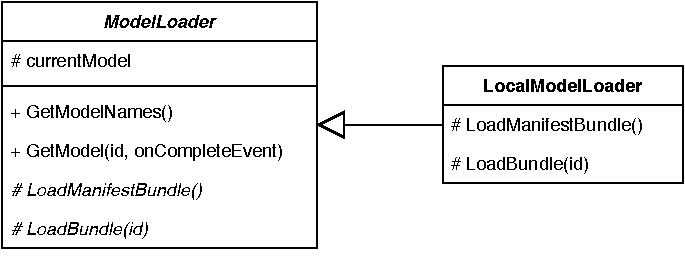
\includegraphics[width=0.6\textwidth]{images/UML-CModelLoader.pdf}
            \caption{Загрузчик моделей.}
            \label{figure:CModelLoader}
        \end{figure}

        Как видно из схемы, для загрузки используется абстрактный класс ModelLoader,
        обладающий двумя публичными методами: метод, позволяющий получить список
        доступных для загрузки информационных моделей, и метод,
        асинхронно загружающий выбранную информационную модель по ее индикатору.
        Для непосредственной загрузки списка доступных моделей и самих моделей
        используются два внутренних метода, реализуемые в подклассах ModelLoader'а.
        Например в рамках прототипа будет реализован класс LocalModelLoader,
        загружающий информационные модели с локального дискового устройства,
        что подробнее рассмотрено в разделе~\ref{subsections:ClientImpl}.
    } 
    \item {
        Размещение модели в виртуальной среде.

        После загрузки модель должна размещаться в виртуальной сцене.
        Для визуализации будет использоваться виртуальный стол,
        на который будет проецироваться модель здания
        в уменьшенном масштабе согласно схеме на рисунке~\ref{figure:CStand}.

        \begin{figure}[ht]
            \centering
            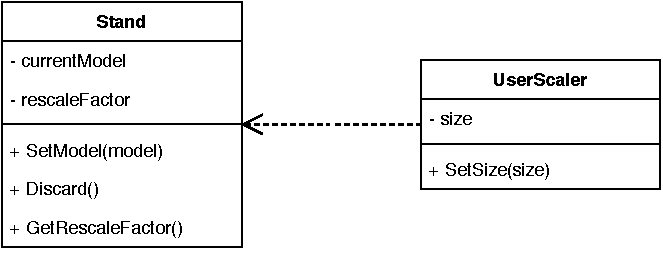
\includegraphics[width=0.6\textwidth]{images/UML-CStand.pdf}
            \caption{Размещение модели.}
            \label{figure:CStand}
        \end{figure}

        Для корректного размещения модели используется класс Stand,
        отвечающий за расчет размеров модели. Размещаемая модель должна
        полностью использовать поверхность виртуального стола,
        не выходя за его пределы. После размещения модели пользователь приложения
        имеет возможность изменять свой размер в виртуальном пространстве,
        чтобы соответствовать размерам модели.
        Для этого используется класс UserScaler, позволяющий изменять размер
        пользователя через передачу числового параметра от 0 до 1,
        где 0 соответствует масштабу информационной модели,
        а 1 -- изначальному размеру пользователя в виртуальной среде.
        Подробности реализации описаны в разделе~\ref{subsections:ClientImpl}.
    } 
    \item {
        Взаимодействие с элементами модели.

        После размещения модель будет разбивать на слои,
        представляющие отдельные структурные элементы здания,
        например стены, лестницы или двери.
        На каждый отдельный слой может накладываться эффект,
        изменяющий его отображение.
        На рисунке~\ref{figure:CLayers} показана
        структура системы слоев.

        \begin{figure}[ht]
            \centering
            \includegraphics[width=0.6\textwidth]{example-image}
            \caption{Система слоев.}
            \label{figure:CLayers}
        \end{figure}

        \intextcomment{
            Описание UML-схемы...
        }
    } 
\end{itemize}

\comment{
    TODO:

    Запилить UML!
}
